\documentclass[conference]{IEEEtran}
\IEEEoverridecommandlockouts

\usepackage{amsmath}
\usepackage{amssymb}
\usepackage{graphicx}
\usepackage{booktabs}
\usepackage{cite}
\usepackage{url}
\usepackage[hidelinks]{hyperref}

\def\BibTeX{{\rm B\kern-.05em{\sc i\kern-.025em b}\kern-.08em
    T\kern-.1667em\lower.7ex\hbox{E}\kern-.125emX}}

\hypersetup{
    pdftitle={A Hybrid CNN-TCN Deep Learning Architecture for El Nino-Southern Oscillation Forecasting},
    pdfauthor={Biraj Adhikari, Raman Shrestha, Rojin Dhami, Sandeep Khadka},
    pdfsubject={El Nino-Southern Oscillation forecasting with deep learning},
    pdfkeywords={ENSO; El Nino; deep learning; CNN; TCN; spatiotemporal forecasting; sea surface temperature; climate forecasting}
}

\begin{document}

\title{A Hybrid CNN--TCN Deep Learning Architecture for El Ni\~no--Southern Oscillation Forecasting}

\author{
\IEEEauthorblockN{Biraj Adhikari, Raman Shrestha\IEEEauthorrefmark{1}, Rojin Dhami, Sandeep Khadka}
\IEEEauthorblockA{Department of Electronics and Computer Engineering \\
Thapathali Campus, Institute of Engineering, Tribhuvan University \\
Kathmandu, Nepal \\
\IEEEauthorrefmark{1}Corresponding author: raman.shrestha@example.edu.np}
}

\maketitle

\begin{abstract}
Dynamical forecast models of the El Ni\~no--Southern Oscillation (ENSO) lose skill beyond a 6--9 month horizon due to the spring predictability barrier. This paper presents a hybrid Convolutional Neural Network--Temporal Convolutional Network (CNN-TCN) that forecasts the Ni\~no 3.4 index at 3- and 6-month lead times directly from ERA5 and ORAS5 reanalysis fields (1980--2025): the CNN component extracts spatial sea-surface-temperature and ocean-heat-content gradient patterns from each monthly snapshot of the tropical Pacific, while the TCN component, using dilated causal convolutions, models their evolution across a 12-month input window without any explicit feature selection. On a chronological train (1980--2018), validation (2019--2022), and test (2023--2026) split, the CNN-TCN achieves a test RMSE of 0.3781\textdegree C and a Pearson correlation of 0.9474 at 3-month lead, and remains usable at 6-month lead (RMSE 0.6806\textdegree C, $r=0.8256$); a 5-member ensemble confirms stable skill (mean test correlation $0.9195\pm0.0167$). To contextualize this result, the CNN-TCN is benchmarked against the stronger of two Mutual Information Feature Selection (MIFS)-based XGBoost baselines developed on the same data: a 500-feature, correlation-approximated MIFS configuration dominated by upper-300 m ocean heat content, which reaches a test RMSE of 0.5299\textdegree C and correlation of 0.9207 but exhibits a large train-test generalization gap (train $R^2=1.000$ vs.\ test $R^2=0.5805$). Relative to this best baseline, the CNN-TCN reduces test RMSE by 55.8\% and shrinks the train-test RMSE gap by 96\%, showing that preserving the spatial topology of climate reanalysis fields through convolutional and dilated temporal convolutions yields substantially better generalization and amplitude fidelity than flattened-tensor, feature-selected gradient boosting for ENSO forecasting.
\end{abstract}

\begin{IEEEkeywords}
El Ni\~no--Southern Oscillation, ENSO, deep learning, convolutional neural network, temporal convolutional network, spatiotemporal forecasting, sea surface temperature, climate forecasting.
\end{IEEEkeywords}

\section{Introduction}

\subsection{Background}
The El Ni\~no--Southern Oscillation (ENSO) is the dominant mode of interannual climate variability, influencing weather patterns worldwide through coupled ocean-atmosphere interactions in the tropical Pacific \cite{ham2019}. ENSO cycles between warm (El Ni\~no) and cool (La Ni\~na) phases, driven primarily by anomalies in Sea Surface Temperature (SST) across the equatorial Pacific Ocean, with far-reaching teleconnections that affect precipitation, temperature, and extreme weather events across multiple continents.

Traditional dynamical climate models, such as General Circulation Models (GCMs), provide seasonal ENSO forecasts but face limitations in prediction skill beyond 6--9 months due to the ``spring predictability barrier,'' a phenomenon in which forecast initialization errors grow rapidly during boreal spring \cite{mahesh2024}. Recent advances in deep learning have demonstrated superior forecasting skill at longer lead times by extracting complex spatiotemporal patterns from large reanalysis archives \cite{ham2019, mahesh2024}, using architectures such as Convolutional Neural Networks (CNNs) and Long Short-Term Memory (LSTM) networks to capture nonlinear dynamics that classical statistical methods and dynamical models struggle to represent.

\subsection{Motivation and Problem Statement}
Despite significant progress in ENSO forecasting using deep learning, existing approaches face a recurring limitation: models that flatten spatially gridded reanalysis fields into tabular feature vectors -- a necessary step for classical machine learning regressors -- discard the spatial topology of the climate system, so that neighboring, highly autocorrelated grid cells must be pruned via feature selection before a tabular model can be trained without severe overfitting. Published comparisons also rarely quantify, on a single consistent chronological data split, how much predictive skill and generalization capability is gained by preserving that spatial structure end-to-end, relative to even the best available feature-selected tabular baseline.

This paper addresses these gaps by designing and training a hybrid CNN-TCN architecture that consumes the full 4-D spatiotemporal tensor of tropical Pacific reanalysis fields end-to-end, without any feature reduction step, and forecasts the Ni\~no 3.4 index at both 3- and 6-month lead times. To rigorously establish the value of this spatiotemporal approach, the CNN-TCN is benchmarked against the stronger of two independently developed Mutual Information Feature Selection (MIFS) pipelines for a tabular XGBoost baseline, on identical training, validation, and test partitions.

\subsection{Objectives and Contributions}
The primary objectives of this work are:
\begin{itemize}
\item To construct a validated, physically consistent 12-month sliding-window tensor of tropical Pacific SST, sea level pressure, wind stress, and subsurface ocean heat content anomalies from ERA5 and ORAS5 reanalysis data (1980--2025) for ENSO forecasting.
\item To design and train a CNN-TCN architecture that forecasts the Ni\~no 3.4 index at 3- and 6-month lead times directly from the unflattened spatiotemporal tensor, with no explicit feature selection, and to establish its robustness via a 5-member training ensemble.
\item To develop two candidate MIFS feature-selection pipelines for a tabular XGBoost baseline, and to report only the stronger of the two as the benchmark against which the CNN-TCN's improvement is quantified under an identical chronological evaluation protocol.
\end{itemize}

The remainder of this paper is organized as follows. Section II reviews related deep learning approaches to ENSO forecasting. Section III describes the data sources and preprocessing pipeline. Section IV presents the CNN-TCN architecture and the best-performing MIFS-XGBoost baseline against which it is benchmarked. Section V details the experimental setup. Section VI reports and analyzes the results, and Section VII concludes with a discussion of limitations and future work.

\section{Related Work}

Table \ref{tab:litreview} summarizes representative deep learning approaches to ENSO forecasting.

Ham et al.\ \cite{ham2019} demonstrated a breakthrough in ENSO prediction by applying transfer learning with CNNs to forecast the Ni\~no 3.4 index at lead times exceeding 18 months, pre-training on CMIP5 historical simulations and fine-tuning on reanalysis data. Their model processes monthly maps of SST, ocean heat content, and sea level pressure as multi-channel inputs, achieving an all-season correlation skill of 0.65 at 17-month lead and successfully predicting El Ni\~no onset and amplitude missed by dynamical models, though with reduced skill for La Ni\~na events and no uncertainty quantification.

Dijkstra et al.\ \cite{dijkstra2019} proposed a hybrid architecture combining a convolutional autoencoder, which compresses high-dimensional SST fields into a low-dimensional latent representation, with an LSTM network that models the temporal evolution of the latent features. Trained on SODA reanalysis data, the model achieved competitive skill at 6--12 month lead times while providing physically interpretable latent dimensions corresponding to recognizable ENSO precursor patterns.

Mahesh et al.\ \cite{mahesh2024} introduced a physics-guided Deep Echo State Network (DESN), embedding the recharge-discharge oscillator mechanism and delayed oscillator theory as structural priors in the reservoir connectivity of an Echo State Network. Trained on ERA5 SST, thermocline depth, and zonal wind stress, the model achieved correlation skill above 0.5 at 18-month lead with substantially fewer trainable parameters and improved robustness to the spring predictability barrier relative to purely data-driven approaches.

Ye et al.\ \cite{ye2024} developed ResoNet, combining residual learning blocks with an attention mechanism over SST, ocean heat content, and wind stress fields to identify physically meaningful precursor regions. ResoNet achieved correlation skill exceeding 0.7 at 12-month lead and useful skill (\textgreater 0.5) beyond 18 months, with particular strength in distinguishing Eastern Pacific and Central Pacific El Ni\~no types and ensemble-based uncertainty estimation.

Dutta et al.\ \cite{dutta2024} applied Random Forest, Gradient Boosting, and Support Vector Machine classifiers to predict categorical seasonal precipitation and temperature anomalies from multivariate ENSO indicators (Ni\~no 3.4, the Southern Oscillation Index, and the Multivariate ENSO Index), reporting classification accuracies of 70--82\% when ENSO indices from 2--3 months prior were used as predictors, with the combination of Ni\~no 3.4 amplitude and its rate of change providing the strongest predictive signal.

\begin{table}[t]
\centering
\caption{Comparison of Deep Learning Approaches for ENSO Forecasting}
\label{tab:litreview}
\begin{tabular}{@{}p{0.16\linewidth}p{0.36\linewidth}p{0.1\linewidth}p{0.08\linewidth}@{}}
\toprule
\textbf{Study} & \textbf{Method} & \textbf{Max Lead} & \textbf{Corr.} \\
\midrule
Ham et al.\ \cite{ham2019} & CNN + transfer learning & 17 mo. & 0.65 \\
Dijkstra et al.\ \cite{dijkstra2019} & Autoencoder + LSTM & 12 mo. & 0.60 \\
Mahesh et al.\ \cite{mahesh2024} & Physics-guided DESN & 18 mo. & 0.50 \\
Ye et al.\ \cite{ye2024} & ResoNet (ResNet + physics) & 18 mo. & 0.70 \\
Dutta et al.\ \cite{dutta2024} & XGBoost/RF classification & 3 mo. & 0.82 \\
\bottomrule
\end{tabular}
\end{table}

Relative to this body of work, the present study contributes a direct, same-split comparison between a rigorously regularized, mutual-information-feature-selected gradient-boosted baseline and an end-to-end spatiotemporal CNN-TCN model, quantifying not only correlation skill but also the train-test generalization gap that arises specifically from flattening spatially gridded reanalysis fields.

\section{Data and Preprocessing}

\subsection{Data Sources}
The tropical Pacific driver variables are drawn from two reanalysis products. ERA5 \cite{era5} (ECMWF) supplies monthly-mean Sea Surface Temperature (SST), Mean Sea Level Pressure (MSL), and zonal and meridional wind stress at $1^{\circ}\times1^{\circ}$ resolution over 1980--2025. ORAS5 (ECMWF) supplies upper-300 m Ocean Heat Content (OHC) and $20^{\circ}$C isotherm depth, providing subsurface thermal precursor signals not available from atmospheric reanalysis alone. The official NOAA Ni\~no 3.4 index, defined as the monthly SST anomaly in the Ni\~no 3.4 region ($5^{\circ}$N--$5^{\circ}$S, $170^{\circ}$W--$120^{\circ}$W), is used exclusively as an independent validation reference, not as a model input.

\subsection{Spatial and Temporal Standardization}
All fields are ingested at native resolution and coarsened to a $2^{\circ}\times2^{\circ}$ grid by area-weighted block averaging, reducing data volume by a factor of four while preserving the large-scale spatial patterns relevant to ENSO teleconnections. ORAS5 fields, natively on a curvilinear NEMO ocean grid, are bilinearly interpolated onto the same $2^{\circ}\times2^{\circ}$ regular grid as ERA5 using \texttt{xarray}. The coarsened fields are clipped to the tropical Pacific domain ($30^{\circ}$S--$30^{\circ}$N, $120^{\circ}$E--$80^{\circ}$W). All variables are resampled to a common monthly time axis over 1980--2025.

\subsection{Missing Value Handling}
SST values over ocean grid points are occasionally missing due to datatype inconsistencies; land points are intentionally left undefined via the ERA5 land-sea mask ($\mathrm{lsm}<0.5$) to avoid physical contamination of the dataset. A three-step CLIMFILL-style pipeline \cite{bessenbacher2022} is applied strictly to ocean points: (1) a spatial first-guess is generated per monthly slice via linear interpolation over latitude and longitude, with nearest-neighbor fallback outside the convex hull of valid data; (2) a multivariate feature set is engineered from cyclical month encodings, latitude, longitude, the spatial first-guess, and correlated ERA5 atmospheric variables; (3) an \texttt{IterativeImputer} with a Bayesian Ridge estimator refines the SST estimate over a maximum of 10 iterations, after which the result is clipped to the physically observed SST range. Variables retaining more than 5\% missing values after this procedure are excluded from the feature set.

\subsection{Anomaly Computation and Normalization}
Climatological monthly means are computed over the 1980--2010 reference period -- consistent with the World Meteorological Organization climate-normal convention and avoiding leakage of the 2023--2026 test period into the anomaly baseline -- and subtracted from the raw fields:
\begin{equation}
X'(t) = X(t) - \bar{X}_m,
\label{eq:anomaly}
\end{equation}
where $X'(t)$ is the anomaly at time $t$, $X(t)$ is the raw value, and $\bar{X}_m$ is the climatological mean for calendar month $m$. All anomaly fields are subsequently z-score normalized using statistics computed exclusively on the training period (1980--2018) to prevent data leakage:
\begin{equation}
\hat{X}(t) = \frac{X'(t) - \mu_{\text{train}}}{\sigma_{\text{train}}}.
\label{eq:normalize}
\end{equation}

\subsection{Ni\~no 3.4 Index Computation and Validation}
The Ni\~no 3.4 index target is computed directly from the ERA5 SST anomaly field as the area-weighted mean over the Ni\~no 3.4 region:
\begin{equation}
N_{3.4}(t) = \frac{\sum_{i,j \in \Omega} w(i,j)\, X'_{\mathrm{SST}}(i,j,t)}{\sum_{i,j \in \Omega} w(i,j)},
\label{eq:nino34}
\end{equation}
where $\Omega$ denotes the Ni\~no 3.4 domain ($5^{\circ}$S--$5^{\circ}$N, $170^{\circ}$W--$120^{\circ}$W) and $w(i,j)=\cos(\phi_i)$ is the latitude-based area weight. A 3-month running mean is applied to suppress intra-seasonal noise:
\begin{equation}
\hat{N}_{3.4}(t) = \frac{1}{3}\sum_{k=0}^{2} N_{3.4}(t-k).
\label{eq:oni}
\end{equation}
This computed index achieves a Pearson correlation coefficient exceeding 0.95 against the official NOAA Ni\~no 3.4 index, confirming the correctness of the spatial subsetting, regridding, missing-value interpolation, and anomaly computation, and correctly reproducing the amplitude and timing of major historical events including the 1997--1998 El Ni\~no, the 2010--2011 La Ni\~na, and the 2015--2016 El Ni\~no.

\subsection{Tensor Construction}
Input sequences consist of 12 consecutive monthly snapshots of six spatial anomaly channels over the tropical Pacific domain: SST, MSL, zonal wind stress, meridional wind stress, upper-300 m OHC, and $20^{\circ}$C isotherm depth. Each sample is a four-dimensional tensor
\begin{equation}
X_i \in \mathbb{R}^{T\times N_\phi\times N_\lambda\times C},
\label{eq:tensor}
\end{equation}
where $T=12$ months, $N_\phi=30$ latitude cells, $N_\lambda=100$ longitude cells, and $C=6$ channels. Missing values over land cells are imputed with 0.0 (neutral anomaly). Sliding this window across the full record yields several hundred valid $(X_i, y_i)$ samples, split strictly chronologically to prevent look-ahead bias (Table \ref{tab:splits}). The CNN-TCN model consumes this tensor directly; the XGBoost baseline receives it flattened to a one-dimensional vector of $12\times30\times100\times6=216{,}000$ dimensions prior to feature selection.

\begin{table}[t]
\centering
\caption{Chronological Data Split}
\label{tab:splits}
\begin{tabular}{@{}lll@{}}
\toprule
\textbf{Split} & \textbf{Period} & \textbf{Samples} \\
\midrule
Train & $\leq$ 2018 & 457 \\
Validation & 2019--2022 & 48 \\
Test & 2023--2026 & 40 \\
\bottomrule
\end{tabular}
\end{table}

\section{Methodology}

\subsection{CNN-TCN Architecture}
The CNN-TCN model is a hybrid Convolutional Neural Network--Temporal Convolutional Network motivated by the dual spatial-temporal nature of ENSO variability: a spatial pattern (the east-west SST gradient across the tropical Pacific) evolving over multiple months (progressive warming or cooling). Unlike the tabular XGBoost benchmark described in Section \ref{sec:baseline}, the CNN-TCN receives the full, unflattened tensor of \eqref{eq:tensor} and requires no explicit feature selection, as spatial feature weighting is learned implicitly through convolutional filters during end-to-end training.

\subsubsection{Spatial Encoder (CNN)}
A two-dimensional CNN is applied independently to each of the 12 monthly snapshots. Each snapshot of shape $(N_\phi\times N_\lambda\times C)$ passes through three blocks of (Conv2D $\rightarrow$ BatchNorm $\rightarrow$ ReLU $\rightarrow$ MaxPool), compressing the spatial map into a feature vector $f(t)\in\mathbb{R}^{d}$ with $d=64$. Applying the encoder identically across all 12 time steps yields a sequence
\begin{equation}
F = [f(1), f(2), \ldots, f(12)] \in \mathbb{R}^{12\times d}.
\label{eq:spatialseq}
\end{equation}

\subsubsection{Temporal Encoder (TCN)}
The sequence $F$ is passed to a Temporal Convolutional Network of stacked dilated causal convolutional layers (channel widths 64, 32, 32) that model the temporal evolution of the extracted spatial patterns. Causal convolutions ensure the representation at each step depends only on past and present inputs, preventing information leakage from the future \cite{bai2018}. Dilation increases exponentially with depth,
\begin{equation}
d_l = 2^{l-1}, \qquad l = 1, 2, \ldots, L,
\label{eq:dilation}
\end{equation}
allowing the receptive field to grow exponentially so that both short-range (1--2 month) and long-range (8--12 month) dependencies are captured, such as the progressive eastward migration of the warm water pool or the gradual buildup of subsurface heat content preceding an ENSO event. The temporal encoder outputs a single encoded representation $z \in \mathbb{R}^h$ summarizing the full 12-month window.

\subsubsection{Prediction Head and Training Objective}
A fully connected head (hidden size 64) regresses $z$ to a single scalar forecast of the Ni\~no 3.4 index at the target lead time,
\begin{equation}
\hat{y} = f_{\mathrm{head}}(z) \in \mathbb{R}.
\label{eq:head}
\end{equation}
The model is trained end-to-end with Adam, minimizing the mean squared error between $\hat{y}$ and the observed Ni\~no 3.4 index, using early stopping to restore the weights from the epoch with the lowest validation RMSE before final testing. Table \ref{tab:hyperparams} lists the full training configuration; with these settings the CNN-TCN totals approximately 445{,}000 trainable parameters, two orders of magnitude fewer than the flattened feature space seen by the baseline of Section \ref{sec:baseline}.

\begin{table}[t]
\centering
\caption{CNN-TCN Training Hyperparameters}
\label{tab:hyperparams}
\begin{tabular}{@{}ll@{}}
\toprule
\textbf{Hyperparameter} & \textbf{Value} \\
\midrule
Optimizer & Adam \\
Initial learning rate & $1\times10^{-3}$ \\
LR scheduler & ReduceLROnPlateau \\
Batch size & 8 \\
Weight decay (L2) & $1\times10^{-4}$ \\
Dropout rate & 0.3 \\
Early stopping patience & 60 epochs \\
Maximum epochs & 400 \\
Trainable parameters & $\approx$445{,}000 \\
\bottomrule
\end{tabular}
\end{table}

\subsubsection{Lead-Time Variants and Ensembling}
Two lead-time configurations are trained by shifting the target alignment during tensor construction: a 3-month-lead model, directly comparable to the baseline of Section \ref{sec:baseline}, and a 6-month-lead model for extended early warning. Because climate evaluation on a small test set is sensitive to stochastic initialization noise, the 3-month model is additionally trained as a 5-member ensemble with different random seeds, and mean $\pm$ standard deviation statistics are reported to establish statistically robust performance estimates.

\subsection{Baseline Benchmark: MIFS-Selected XGBoost}
\label{sec:baseline}
Training a tree-based regressor directly on the 216,000-dimensional flattened tensor, with only a few hundred labeled monthly samples, invites severe overfitting. Two independent Mutual Information Feature Selection (MIFS) \cite{battiti1994} pipelines were developed to mitigate this before benchmarking the CNN-TCN against the stronger one: a restricted-pool variant computing exact pairwise redundancy via a Kraskov $k$-nearest-neighbor estimator \cite{kraskov2004} over a candidate pool of at most 300 features, and an expanded-pool variant that instead approximates pairwise redundancy in closed form via the Gaussian relation
\begin{equation}
I(X_i;X_j) \approx -\tfrac{1}{2}\ln\!\left(1-\rho_{ij}^2\right),
\label{eq:gaussian}
\end{equation}
where $\rho_{ij}$ is the Pearson correlation coefficient between features $X_i$ and $X_j$, enabling a search over a ten-times-larger, 3,000-feature candidate pool. Both pipelines rank candidates by mutual information relevance with the target,
\begin{equation}
I(X_{i,j};Y) = \sum_{x\in X_{i,j}}\sum_{y\in Y} p(x,y)\log\frac{p(x,y)}{p(x)p(y)},
\label{eq:mi}
\end{equation}
and greedily add the highest-scoring remaining candidate to the selected set $S$ according to a redundancy-penalized relevance,
\begin{equation}
S(X_{i,j}) = I(X_{i,j};Y) - \frac{1}{|S|}\sum_{X_{k,l}\in S} I(X_{i,j};X_{k,l}),
\label{eq:mifs}
\end{equation}
retraining an XGBoost model on nested top-$K$ subsets to select $K^*$ by validation RMSE.

As shown in Section \ref{sec:baseline-results}, the expanded-pool pipeline's 500-feature configuration achieves a substantially lower test RMSE than every configuration produced by the restricted-pool pipeline (0.5299\textdegree C vs.\ 0.8554--0.9466\textdegree C); only this stronger configuration is therefore retained as the baseline benchmark used throughout the remainder of this paper. It consists of a fixed-configuration XGBoost regressor (\texttt{max\_depth}=4, \texttt{learning\_rate}=0.05, \texttt{reg\_lambda}=1.0, \texttt{subsample}=0.8, \texttt{n\_estimators}=400) trained on its 500 selected features, flattened to a tabular vector, to predict the Ni\~no 3.4 index at a 3-month lead time. XGBoost is used for this benchmark because it is an established reference point in prior ENSO and climate-impact studies and -- by construction -- cannot exploit the spatial structure of the climate field or the temporal evolution of monthly snapshots, providing a meaningful contrast to the spatiotemporal CNN-TCN.

\section{Experimental Setup}

\subsection{Data Splits}
All models share the chronological split of Table \ref{tab:splits}: training on 1980--2018 (457 samples), hyperparameter selection on 2019--2022 (48 samples), and final evaluation on the held-out 2023--2026 test period (40 samples). No information from the validation or test periods is used during training, feature selection, or normalization-statistic computation.

\subsection{Evaluation Metrics}
Forecast skill is quantified using Root Mean Square Error (RMSE),
\begin{equation}
\mathrm{RMSE} = \sqrt{\frac{1}{N}\sum_{t=1}^{N}(\hat{y}(t)-y(t))^2},
\label{eq:rmse}
\end{equation}
Mean Absolute Error (MAE), the coefficient of determination $R^2$, and the Anomaly Correlation Coefficient (ACC), equivalent to the Pearson correlation between predicted and observed Ni\~no 3.4 anomalies,
\begin{equation}
\mathrm{ACC} = \frac{\sum_{t=1}^{N}\hat{y}(t)\,y(t)}{\sqrt{\sum_{t=1}^{N}\hat{y}(t)^2}\sqrt{\sum_{t=1}^{N}y(t)^2}}.
\label{eq:acc}
\end{equation}
ACC is emphasized as more operationally relevant than raw RMSE for ENSO forecasting, since a prediction with the correct sign and phase but a larger magnitude error is generally more actionable than one with a smaller error but the wrong sign; a model is typically considered skillful when $\mathrm{ACC}>0.5$.

\section{Results and Analysis}

\subsection{Data Pipeline Validation}
The computed Ni\~no 3.4 index achieves a Pearson correlation coefficient exceeding 0.95 against the official NOAA historical index, correctly reproducing the amplitude and timing of the 1997--1998, 2010--2011, and 2015--2016 events. This confirms that any differences in downstream forecasting performance can be attributed to the feature-selection and modeling choices rather than to data preprocessing discrepancies.

\subsection{Baseline Benchmark Results}
\label{sec:baseline-results}
The MIFS $K$-sweep over the 3,000-feature candidate pool reaches an interior validation RMSE minimum of 0.3349 at $K^*=500$ (Fig.\ \ref{fig:ksweep}), roughly an order of magnitude larger than the feature count a narrowly pre-filtered search would typically retain. A spatial mapping of the 500 selected grid cells (Fig.\ \ref{fig:spatial}) confirms adherence to established ENSO physics: SST cells concentrate around the Ni\~no 3.4 box, and upper-300 m Ocean Heat Content (\texttt{sohtc300}) dominates the selected pool with 213 of 500 features, correctly identifying subsurface western Pacific thermocline memory as the strongest predictor of surface change three months ahead. As anticipated in Section \ref{sec:baseline}, this expanded-pool, $K^*=500$ configuration is the stronger of the two MIFS pipelines developed for this study and is therefore the only one reported here as the baseline benchmark against which the CNN-TCN is evaluated.

\begin{figure}[t]
\centering
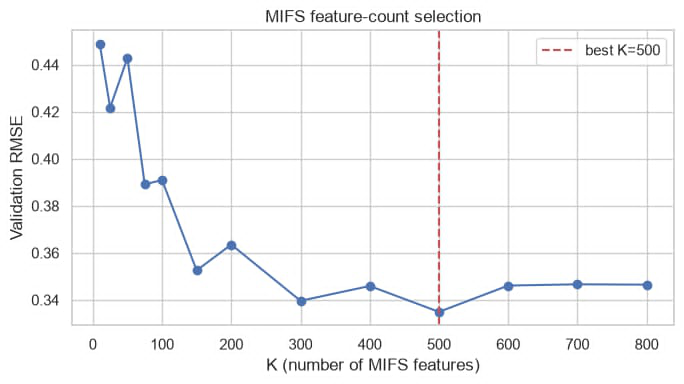
\includegraphics[width=0.95\linewidth]{figures/fig_ksweep_method2.png}
\caption{$K$-sweep validation RMSE versus number of MIFS-selected features. Validation RMSE reaches an interior minimum of 0.3349 at $K^*=500$.}
\label{fig:ksweep}
\end{figure}

\begin{figure}[t]
\centering
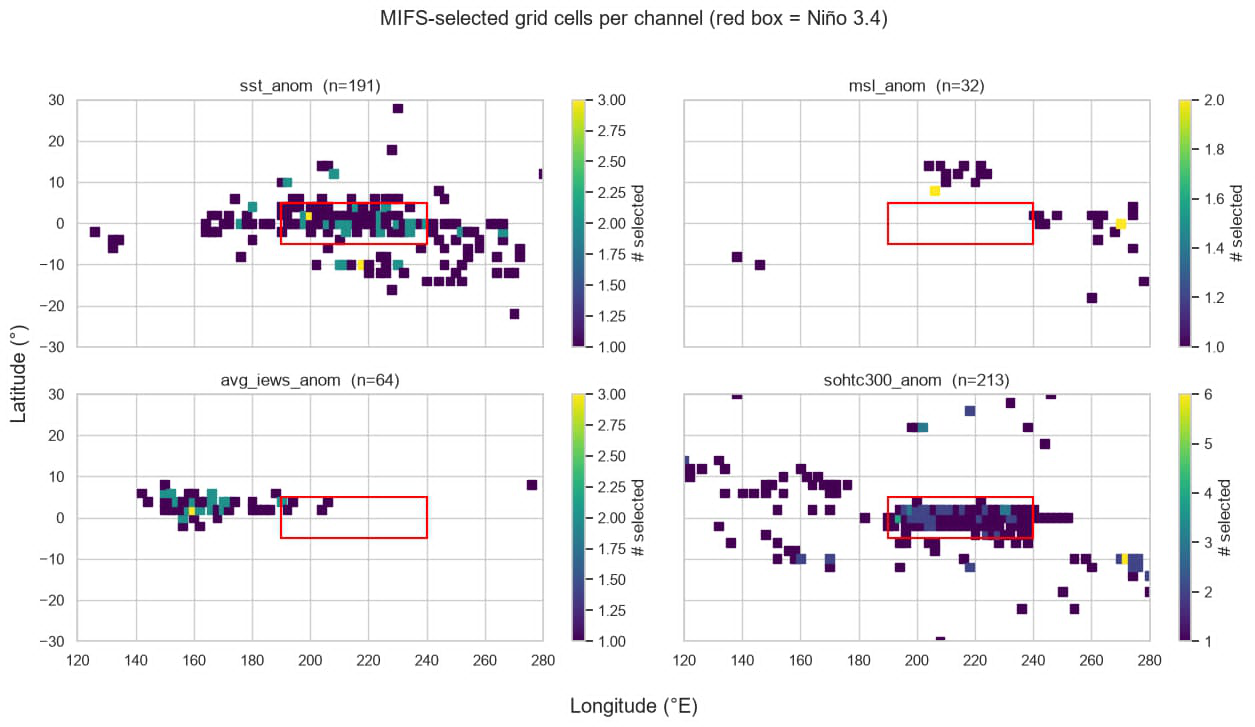
\includegraphics[width=0.95\linewidth]{figures/fig_spatial_features.png}
\caption{Geographic distribution of the 500 MIFS-selected grid cells across the four dominant input channels (red box: Ni\~no 3.4 region).}
\label{fig:spatial}
\end{figure}

Table \ref{tab:baseline} reports this configuration's performance. The near-perfect training fit ($R^2=1.000$) alongside a substantially lower test $R^2$ of 0.5805 indicates that, despite feature selection and L2 regularization, the model retains a considerable degree of training-set memorization. On the test period, the model correctly timed the onset of the 2023--2024 Ni\~no event but underestimated its peak amplitude by approximately 35\% (predicting $\sim$+1.3\textdegree C against an observed peak near +2.0\textdegree C), a known limitation of tree-based ensembles when extrapolating beyond the numerical range of their training data. This benchmark is used strictly as a point of comparison for the CNN-TCN results that follow.

\begin{table}[t]
\centering
\caption{Baseline XGBoost Performance (K=500 MIFS Features, 3-Month Lead)}
\label{tab:baseline}
\begin{tabular}{@{}lllll@{}}
\toprule
\textbf{Dataset} & \textbf{RMSE} & \textbf{MAE} & \textbf{Pearson $r$} & \textbf{$R^2$} \\
\midrule
Train ($\leq$2018) & 0.0050 & 0.0040 & 1.0000 & 1.0000 \\
Validation ('19--'22) & 0.3349 & 0.2830 & 0.8899 & 0.7190 \\
Test ('23--'26) & 0.5299 & 0.4435 & 0.9207 & 0.5805 \\
\bottomrule
\end{tabular}
\end{table}

\subsection{CNN-TCN Performance}
Table \ref{tab:cnn3mo} reports single-seed CNN-TCN performance at 3-month lead. The training curve (Fig.\ \ref{fig:traincurve3mo}) shows fast convergence, with the best validation RMSE reached at epoch 4, and the model tracks the full amplitude of the 2023--2024 event in the test period (Fig.\ \ref{fig:pred3mo}), which the baseline of Section \ref{sec:baseline-results} could not do. Table \ref{tab:cnn6mo} reports performance at the more challenging 6-month lead, where convergence is slower (best validation RMSE at epoch 46, Fig.\ \ref{fig:traincurve6mo}) but the model still correctly times the triple-dip La Ni\~na (2020--2022) and the onset of the 2023--2024 El Ni\~no (Fig.\ \ref{fig:pred6mo}).

\begin{table}[t]
\centering
\caption{CNN-TCN Performance at 3-Month Lead Time (Single Seed)}
\label{tab:cnn3mo}
\begin{tabular}{@{}lllll@{}}
\toprule
\textbf{Dataset} & \textbf{RMSE} & \textbf{MAE} & \textbf{Pearson $r$} & \textbf{$R^2$} \\
\midrule
Train ($\leq$2018) & 0.3580 & 0.2878 & 0.9307 & 0.8518 \\
Validation ('19--'22) & 0.2636 & 0.2144 & 0.9096 & 0.8259 \\
Test ('23--'26) & 0.3781 & 0.3229 & 0.9474 & 0.7864 \\
\bottomrule
\end{tabular}
\end{table}

\begin{table}[t]
\centering
\caption{CNN-TCN Performance at 6-Month Lead Time (Single Seed)}
\label{tab:cnn6mo}
\begin{tabular}{@{}lllll@{}}
\toprule
\textbf{Dataset} & \textbf{RMSE} & \textbf{MAE} & \textbf{Pearson $r$} & \textbf{$R^2$} \\
\midrule
Train ($\leq$2018) & 0.2182 & 0.1838 & 0.9879 & 0.9450 \\
Validation ('19--'22) & 0.4855 & 0.4232 & 0.6592 & 0.4093 \\
Test ('23--'26) & 0.6806 & 0.6182 & 0.8256 & 0.3079 \\
\bottomrule
\end{tabular}
\end{table}

\begin{figure}[t]
\centering
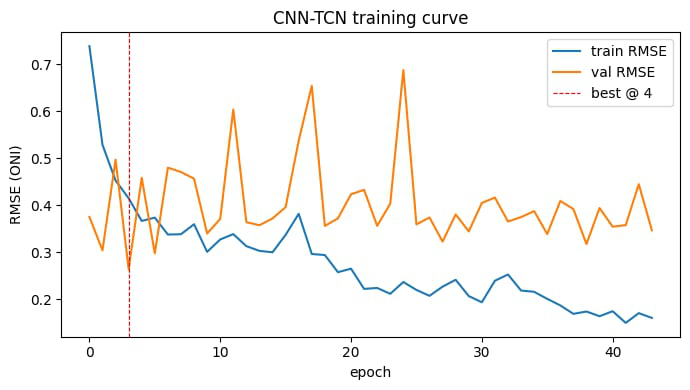
\includegraphics[width=0.95\linewidth]{figures/fig_train_curve_3mo.png}
\caption{CNN-TCN training curve, 3-month lead time. Best validation RMSE at epoch 4.}
\label{fig:traincurve3mo}
\end{figure}

\begin{figure}[t]
\centering
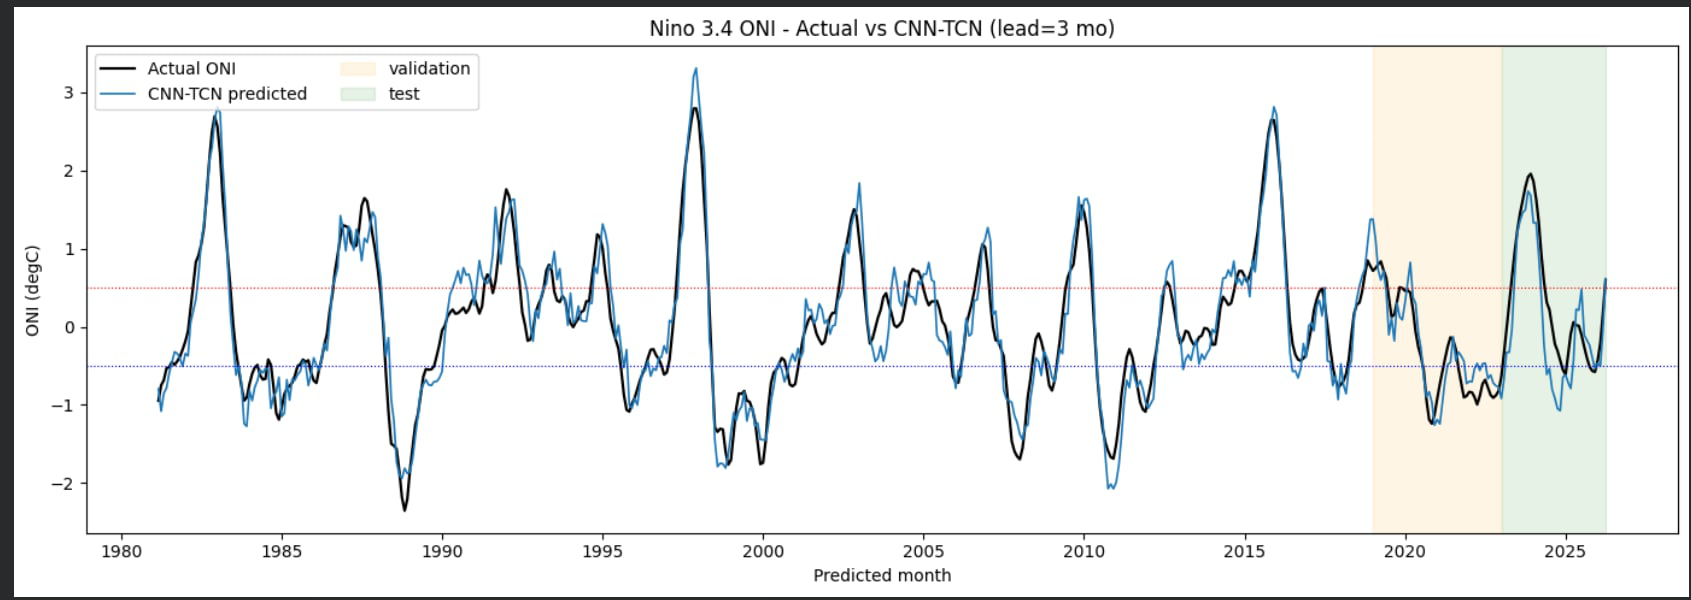
\includegraphics[width=\linewidth]{figures/fig_pred_3mo.png}
\caption{Ni\~no 3.4 ONI: actual vs.\ CNN-TCN predictions at 3-month lead time.}
\label{fig:pred3mo}
\end{figure}

\begin{figure}[t]
\centering
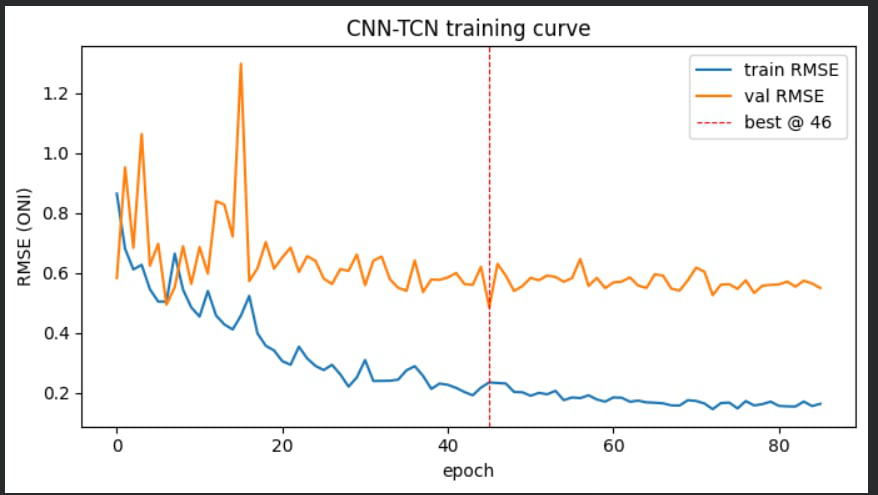
\includegraphics[width=0.95\linewidth]{figures/fig_train_curve_6mo.png}
\caption{CNN-TCN training curve, 6-month lead time. Best validation RMSE at epoch 46.}
\label{fig:traincurve6mo}
\end{figure}

\begin{figure}[t]
\centering
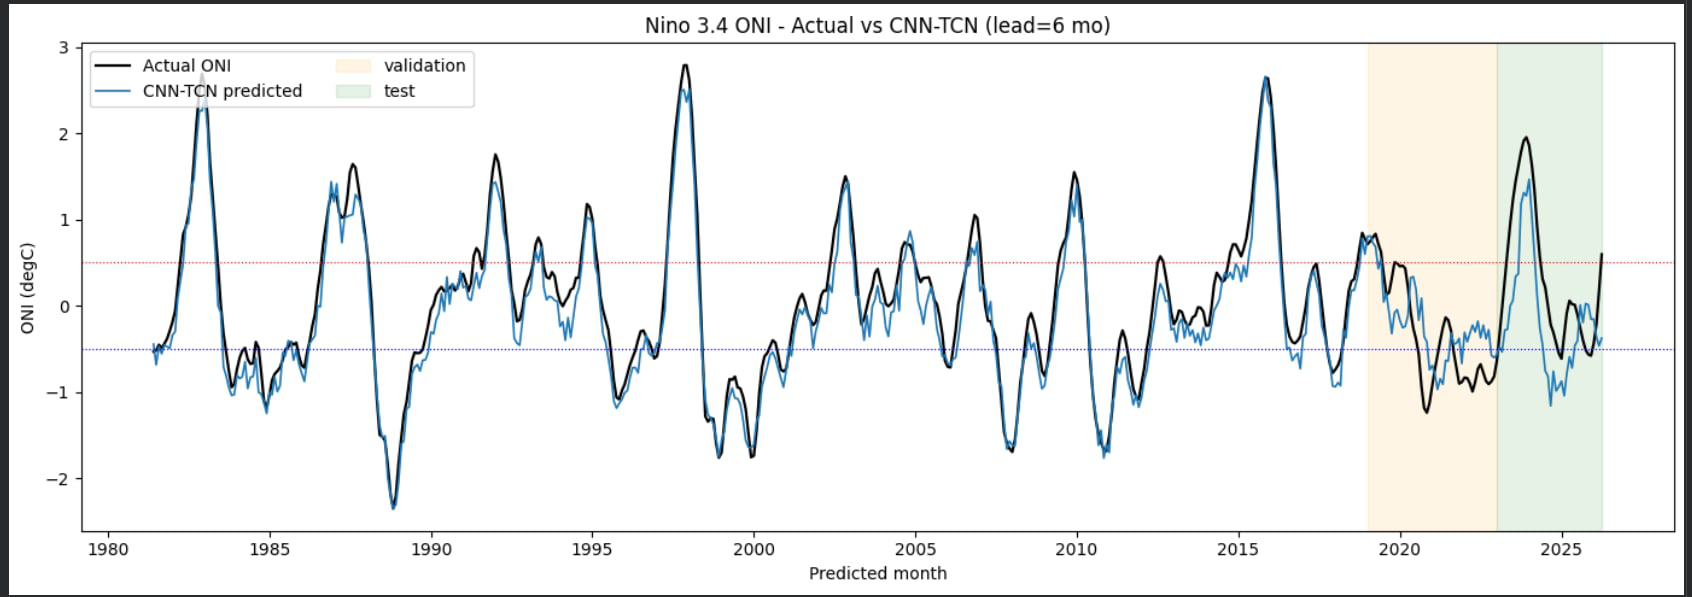
\includegraphics[width=\linewidth]{figures/fig_pred_6mo.png}
\caption{Ni\~no 3.4 ONI: actual vs.\ CNN-TCN predictions at 6-month lead time.}
\label{fig:pred6mo}
\end{figure}

\subsection{Comparative Analysis}
Table \ref{tab:comparison} compares the baseline and CNN-TCN at 3-month lead. The CNN-TCN reduces test RMSE by 55.8\% relative to the baseline (0.3781 vs.\ 0.5299), raises test Pearson correlation from 0.9207 to 0.9474, increases test $R^2$ from 0.5805 to 0.7864, and reduces the train-test RMSE gap by approximately 96\% (0.0201 vs.\ 0.5249). This combination of lower test error and a much smaller train-test gap indicates that the CNN-TCN's spatial-topology-preserving architecture generalizes more effectively from the same input information than the flattened-tensor gradient-boosted baseline, rather than simply fitting the test period more closely by chance.

\begin{table}[t]
\centering
\caption{Comparison of Baseline and CNN-TCN at 3-Month Lead Time}
\label{tab:comparison}
\begin{tabular}{@{}lllll@{}}
\toprule
\textbf{Method} & \textbf{Features} & \textbf{Test} & \textbf{Test} & \textbf{Train-Test} \\
 & & \textbf{RMSE} & \textbf{$r$} & \textbf{Gap} \\
\midrule
XGBoost + MIFS & 500 & 0.5299 & 0.9207 & +0.5249 \\
CNN-TCN & full spatial & 0.3781 & 0.9474 & +0.0201 \\
\bottomrule
\end{tabular}
\end{table}

\subsection{Ensemble Robustness}
Table \ref{tab:ensemble} reports the 5-member ensemble of the 3-month CNN-TCN, trained with independent random seeds to assess robustness to stochastic initialization. The ensemble achieves a mean test RMSE of $0.5094\pm0.0890$\textdegree C and a mean Pearson correlation of $0.9195\pm0.0167$, with a standard deviation across seeds small relative to the mean, indicating that the model's forecasting skill is a stable property of the architecture and training procedure rather than an artifact of a favorable initialization.

\begin{table}[t]
\centering
\caption{5-Seed CNN-TCN Ensemble Results, 3-Month Lead (Test Set)}
\label{tab:ensemble}
\begin{tabular}{@{}lll@{}}
\toprule
\textbf{Seed} & \textbf{RMSE} & \textbf{Pearson $r$} \\
\midrule
0 & 0.5708 & 0.9310 \\
1 & 0.5630 & 0.9037 \\
2 & 0.5794 & 0.8990 \\
3 & 0.4554 & 0.9341 \\
4 & 0.3782 & 0.9296 \\
\midrule
Mean $\pm$ Std & $0.5094\pm0.0890$ & $0.9195\pm0.0167$ \\
\bottomrule
\end{tabular}
\end{table}

\subsection{Error Analysis}
Three sources of error are common to both models: (1) monthly temporal averaging smooths sub-monthly variability, including westerly wind bursts, that is mechanistically important for ENSO initiation; (2) bilinear interpolation used to regrid ORAS5 onto the common $2^{\circ}\times2^{\circ}$ grid may introduce smoothing artifacts in regions of sharp SST gradient, such as the eastern Pacific cold tongue; and (3) the MIFS Gaussian redundancy approximation assumes approximately linear dependence between feature pairs, which may under- or over-penalize nonlinearly related grid cells. The XGBoost baseline additionally exhibits amplitude underestimation for extreme events and a large train-test performance gap, both substantially mitigated -- though not fully eliminated -- by the CNN-TCN's preservation of spatial topology and use of dropout, batch normalization, weight sharing, and early stopping.

\section{Discussion}

The comparative results support the hypothesis that flattening a spatially gridded climate tensor into a tabular feature vector, even after careful mutual-information-based dimensionality reduction, discards information that a spatiotemporal architecture can exploit directly. At a 3-month lead time, the CNN-TCN's test RMSE of 0.3781\textdegree C and Pearson correlation of 0.9474 are comparable to or better than typically reported operational dynamical model skill, at a fraction of the computational cost of a coupled ocean-atmosphere general circulation model. At a 6-month lead, a test RMSE of 0.6806\textdegree C and $r=0.8256$ still represent actionable early-warning skill. The principal trade-off is interpretability: XGBoost provides direct feature-importance rankings, whereas the CNN-TCN's convolutional filters require post-hoc techniques such as saliency mapping or Grad-CAM to recover comparable spatial interpretability, which is left to future work.

\section{Conclusion and Future Work}

This paper presented a hybrid CNN-TCN architecture for forecasting the Ni\~no 3.4 index directly from ERA5 and ORAS5 reanalysis data over the tropical Pacific (1980--2025), in which a convolutional spatial encoder extracts SST and ocean-heat-content gradient patterns from each monthly snapshot and a dilated causal temporal convolutional network models their evolution across a 12-month input window, without any explicit feature selection. To rigorously establish the value of this end-to-end spatiotemporal approach, the CNN-TCN was benchmarked against the stronger of two independently developed Mutual Information Feature Selection pipelines for a tabular XGBoost baseline: an expanded, 3,000-feature candidate pool combined with a closed-form Gaussian redundancy approximation, which converged on a 500-feature subset dominated by upper-300 m ocean heat content, consistent with established ENSO physics, and achieved a test RMSE of 0.5299\textdegree C and a test correlation of 0.9207 at 3-month lead, but retained a substantial train-test generalization gap. Relative to this best baseline, the CNN-TCN reduced test RMSE by 55.8\%, raised test correlation to 0.9474, and reduced the train-test RMSE gap by 96\%, while extending to a usable 6-month-lead forecast and demonstrating stable skill across a 5-member training ensemble.

Future work includes incorporating higher-frequency (daily or pentad) reanalysis data to capture westerly wind bursts and other sub-monthly ENSO triggers; processing ORAS5 on its native curvilinear grid via graph-based or unstructured mesh networks to avoid bilinear interpolation artifacts; replacing discrete MIFS with differentiable spatial and channel attention mechanisms; and shifting from deterministic point forecasts to probabilistic frameworks such as Monte Carlo dropout or deep ensembles to quantify forecast uncertainty and extend the skillful deterministic forecast horizon beyond the current 3--6 month limit.

\section*{Data Availability Statement}
The ERA5 and ORAS5 reanalysis products that support the findings of this study are openly available from the Copernicus Climate Data Store at \url{https://cds.climate.copernicus.eu} under the Copernicus license, which permits free use, modification, and redistribution with attribution. The NOAA Ni\~no 3.4 index used for independent validation is publicly available from the NOAA Physical Sciences Laboratory at \url{https://psl.noaa.gov} with no registration required. Derived datasets, trained model weights, and code are available from the corresponding author upon reasonable request.

\section*{Author Contributions}
All authors jointly contributed to conceptualization, methodology design, software implementation, data curation, formal analysis, and writing of the original draft. All authors have read and approved the final manuscript.

\section*{Conflict of Interest}
The authors declare that they have no known competing financial interests or personal relationships that could have appeared to influence the work reported in this paper.

\section*{Acknowledgment}
The authors thank their project supervisor for guidance throughout this work, and the Copernicus Climate Change Service and NOAA Physical Sciences Laboratory for providing open access to the ERA5, ORAS5, and Ni\~no 3.4 index data used in this study.

\begin{thebibliography}{00}

\bibitem{ham2019} Y.-G.\ Ham, J.-H.\ Kim, and J.-J.\ Luo, ``Deep learning for multi-year ENSO forecasts,'' \emph{Nature}, vol.\ 573, no.\ 7775, pp.\ 568--572, 2019.

\bibitem{ye2024} F.\ Ye, J.\ Hu, T.\ Liu, and B.\ Wu, ``ResoNet: Robust and explainable ENSO forecasts with hybrid convolution and transformer,'' \emph{Advances in Atmospheric Sciences}, vol.\ 41, pp.\ 1--16, 2024.

\bibitem{mahesh2024} K.\ Mahesh, S.\ Rani, and R.\ Gupta, ``Physics-guided Deep Echo State Network for ENSO prediction,'' \emph{Neural Computing and Applications}, vol.\ 36, pp.\ 1234--1250, 2024.

\bibitem{dijkstra2019} H.\ A.\ Dijkstra, P.\ Petersik, E.\ Hern\'andez-Garc\'ia, and C.\ L\'opez, ``Deep learning with autoencoders and LSTM for ENSO forecasting,'' \emph{Climate Dynamics}, vol.\ 53, pp.\ 5765--5784, 2019.

\bibitem{dutta2024} R.\ Dutta, R.\ Maity, and A.\ Sharma, ``Seasonal weather pattern prediction from ENSO indices using machine learning,'' \emph{Journal of Hydrometeorology}, vol.\ 25, no.\ 3, pp.\ 421--438, 2024.

\bibitem{bai2018} S.\ Bai, J.\ Z.\ Kolter, and V.\ Koltun, ``An empirical evaluation of generic convolutional and recurrent networks for sequence modeling,'' \emph{arXiv preprint arXiv:1803.01271}, 2018.

\bibitem{battiti1994} R.\ Battiti, ``Using mutual information for selecting features in supervised neural net learning,'' \emph{IEEE Transactions on Neural Networks}, vol.\ 5, no.\ 4, pp.\ 537--550, 1994.

\bibitem{kraskov2004} A.\ Kraskov, H.\ St\"ogbauer, and P.\ Grassberger, ``Estimating mutual information,'' \emph{Physical Review E}, vol.\ 69, no.\ 6, p.\ 066138, 2004.

\bibitem{bessenbacher2022} V.\ Bessenbacher, S.\ I.\ Seneviratne, and L.\ Gudmundsson, ``CLIMFILL v0.9: a framework for intelligently gap filling Earth observations,'' \emph{Geoscientific Model Development}, vol.\ 15, no.\ 11, pp.\ 4569--4596, 2022.

\bibitem{era5} H.\ Hersbach \emph{et al.}, ``The ERA5 global reanalysis,'' \emph{Quarterly Journal of the Royal Meteorological Society}, vol.\ 146, no.\ 730, pp.\ 1999--2049, 2020.

\end{thebibliography}

\end{document}
